\documentclass[a4paper]{article}
\usepackage[margin = 3cm]{geometry}
\usepackage{babel}
\usepackage[utf8]{inputenc}
\usepackage{amsmath,amsthm}
\usepackage{amssymb}
\usepackage{graphicx, subfig}
\usepackage{tikz}
\usetikzlibrary{positioning, shapes, calc, arrows.meta}
\usepackage{xcolor}
\usepackage{enumitem}
\usepackage[hidelinks]{hyperref}


% bibliography
\usepackage[round]{natbib}

% itemize
\renewcommand{\descriptionlabel}[1]{%
  \hspace\labelsep \upshape\bfseries #1%
}

% example
\theoremstyle{definition}
\newtheorem{example}{Example}
\newtheorem{remark}{Remark}

% referencing description
\makeatletter
\let\orgdescriptionlabel\descriptionlabel
\renewcommand*{\descriptionlabel}[1]{%
  \let\orglabel\label
  \let\label\@gobble
  \phantomsection
  \edef\@currentlabel{#1\unskip}%
  %\edef\@currentlabelname{#1}%
  \let\label\orglabel
  \orgdescriptionlabel{#1}%
}
\makeatother

\DeclareMathOperator{\N}{\mathcal{N}}
\DeclareMathOperator{\KL}{KL}
\DeclareMathOperator{\mise}{MISE}
\DeclareMathOperator{\mse}{MSE}
\DeclareMathOperator{\ent}{Ent}
\newcommand{\norm}[2]{\ensuremath{\Vert #1 \Vert_{#2}}}
\newcommand{\variation}[1]{\ensuremath{\frac{\delta E}{\delta #1}}}

\def\real{\mathbb{R}}
\def\testfn{\varphi}


\title{Solving Fredholm integral equations of the first kind via Wasserstein gradient flow}
\author{Arnaud -> Adam, Francesca }
\date{ }

\begin{document}
\maketitle


% images location
\graphicspath{{Images/}}

\section{Fredholm integral equation of first kind}

We want to solve the integral equation
\[
\mu(y)=\int\rho\left(x\right)K(x,y)dx,
\]
where $\rho$ and $\mu$ are probability densities on $\real^{n}$ and $\real^{m}$ and $K$ a Markov transition density, i.e. $\mu=\rho K$ in operator notation. The solution to this problem is not unique and we propose to regularize the problem using an entropy constraint; i.e. for a given $\lambda>0$ we propose to minimize w.r.t. $\rho$
\begin{equation}
\label{eq:minimisation}
E(\rho)=\KL(\mu,\rho K)-\lambda\ent(\rho)
\end{equation}
where 
$\KL(\mu,\rho K)$ is the Kullback-Leibler divergence between $\mu$ and $\rho K$ and $\ent(\rho)=-\int\rho\log\rho$ is the entropy of $\rho$.
This requires solving a minimization problem in the space of probability measures. We are going to follow a Wasserstein gradient flow approach.

\subsection{Assumptions}
\begin{description}
\item[(A0)\label{a}] $\mu, \rho$ are probability densities with finite second moment and $K$ is a the density of a Markov kernel for each $x$.
\item[(A1)\label{a:k}] the kernel $K(x, y)$ is bounded above and below
\begin{equation*}
 \exists m_K>0 \text{ such that }\qquad 0<  \frac{1}{m_K} \leq  K(x, y)\leq m_K < \infty \qquad \forall (x, y),
\end{equation*}
is convex in $x$ uniformly in $y$ and is Lipschitz continuous in $x$ uniformly in $y$ with Lipschitz constant $L$.
\item[(A2)\label{a:gradientk}] the gradient $\nabla K(x, y)$ is Lipschitz continuous in $x$ uniformly in $y$ with Lipschitz constant $L^\prime$.
\end{description}

\ref{a:k} implies that $\mu$ is bounded too.
\section{Gradient flow approach}
\subsection{Notation}

Let us denote the set of probability measures with finite second moment on $\real^d$ by
\begin{align*}
\mathcal{P}_2(\real^d) = \left\lbrace \mu\in \mathcal{P}(\real^d): \int \norm{ x}{2}^2 \ d\mu(x)< \infty\right\rbrace
\end{align*}
and we define the 2-Wasserstein distance on this set
\begin{align*}
W_2(\mu, \nu) := \left( \inf_{\pi\in\Pi(\mu, \nu)}\int\norm{x - y}{2}\ d\pi(x, y)\right)^{1/2}
\end{align*}
where $\Pi(\mu, \nu)$ is the set of all possible couplings between $\mu$ and $\nu$.

GEODESICALLY CONVEX	

For any proper and lower semicontinuous functional $F$ defined on $\mathcal{P}_2(\real^d)$, $\xi$ belongs to the sub-differential $\partial F(\mu)$ if
\begin{align*}
F(\nu) - F(\mu) \geq \int\langle \xi(x), T(x) - x\rangle\ d\mu(x) +o\left( W_2(\mu, \nu)\right)
\end{align*}
with $T$ transport map from $\mu$ to $\nu$.

\subsection{Properties of the functional $E$}

We consider the functional $E$ in \eqref{eq:minimisation} defined on $\mathcal{P}_2(\real^n)$.

It is easy to see that this functional is geodesically convex in $\rho$.
\begin{proof}
We have
\begin{align*}
E(\rho)= & \KL(\mu,\rho K)-\lambda\ent(\rho)\\
=- & \int\mu\log\rho K+\lambda\int\rho\log\rho+\int\mu\log\mu.
\end{align*}
The integral $\int\mu\log\mu$ is constant w.r.t. $\rho$ and the negative entropy $\lambda\int\rho\log\rho$ is geodesically convex in $\rho$ \citep[page 130]{santambrogio2017euclidean}.
Regarding the integral $- \int\mu\log\rho K$, we have that
\begin{itemize}
\item $\rho K = \int K(x, y) \ d\rho(x)$ is geodesically convex if $K$ is convex in $x$ \citep[page 128]{santambrogio2017euclidean}
\item $-\log s$ is a convex function
\end{itemize}
hence $\int\mu\left( -\log\rho K\right)$ is convex in $\rho$ (integrating w.r.t. $\mu$ does not change convexity).
\end{proof}

The functional $E$ is also continuous in $\left(\mathcal{P}_2(\real^n), W_2\right)$.
\begin{proof}
As $W_2$ metrizes weak convergence, take $\rho_n \rightharpoonup \rho$. Then
\begin{align*}
\vert E(\rho_n) - E(\rho)\vert &= \left\lvert -\int\mu\log\rho_n K+\lambda\int\rho_n\log\rho_n +\int\mu\log\rho K-\lambda\int\rho\log\rho\right\rvert\\
&\leq  \left\lvert \int\mu\left[\log\rho K - \log\rho_n K \right]\right\rvert +\lambda\left\lvert\int\left[ \rho_n\log\rho_n -\rho\log\rho\right]\right\rvert
\end{align*}
if $K$ is continuous, since $\rho_n \rightharpoonup \rho$, we also have that $\rho_n K \rightarrow \rho K$ and the continuity of the logarithm gives $\log\rho K \rightarrow\log\rho_n K$. The dominated convergence theorem gives
\begin{align*}
\left\lvert \int\mu\left[\log\rho K - \log\rho_n K \right]\right\rvert \rightarrow 0.
\end{align*}
Similarly, continuity of the second term is given by the continuity of the entropy function and the dominated convergence theorem.
\end{proof}

\subsection{Gradient flow}
Following \citet[Definition 11.1.1]{ambrosio2008gradient}, we say that $\rho_t$ is a solution to the gradient flow equation for $E$ with the $W_2$ metric if
\begin{equation*}
v_t \in -\partial E(\rho_t),
\end{equation*}
where $\partial E(\rho_t)$ is the sub-differential of $E$ evaluated at $\rho_t$, and $v_t$ is a "gradient" for $E$ at $\rho_t$ such that
\begin{align*}
\partial_{t}\rho_{t}=-\nabla\cdot\left(\rho_{t}v_t\right)
\end{align*} 
holds.

To arrive to an expression for $v_t$ we compute the first variation of $E$
\begin{align*}
\lim_{\epsilon\rightarrow0}\epsilon^{-1}\left(E(\rho+\epsilon\chi)-E(\rho)\right)=\int\frac{\delta E}{\delta\rho}\left(x\right)\chi\left(dx\right),
\end{align*}
where $\chi$ is any signed measure such that $\rho+\epsilon\chi$ is a probability measure, and then we need to show that this is a sub-differential for $E$.
\textcolor{red}{I don't think we can immediately say that the first variation is a sub-differential because $E$ is not a free energy \citep[Lemma 8-10]{carrillo2006contractions}}

\subsubsection{First variation}

We have
\begin{align*}
E(\rho)= & \KL(\mu,\rho K)-\lambda\ent(\rho)\\
=- & \int\mu\log\rho K+\lambda\int\rho\log\rho+\int\mu\log\mu.
\end{align*}
It follows directly that 
\[
\frac{\delta\ent }{\delta\rho}\left(\rho\right)=-(1+\log\rho).
\]
and 
\begin{align*}
\int\mu\log\left(\left(\rho+\epsilon\chi\right)K\right)-\int\mu\log\left(\rho K\right) & =\int\mu\left\{ \log\left(\rho K\right)+\log\left(1+\frac{\epsilon\chi K}{\rho K}\right)\right\} -\int\mu\log\left(\rho K\right)\\
 & =\int\mu\log\left(1+\frac{\epsilon\chi K}{\rho K}\right)\\
 & =\int\mu\left(\frac{\epsilon\chi K}{\rho K}+o\left(\frac{\epsilon\chi K}{\rho K}\right)\right)\\
 & =\epsilon\int\mu\frac{\chi K}{\rho K}+o\left(\epsilon\int\mu\frac{\chi K}{\rho K}\right).
\end{align*}
We have 
\[
\int\mu\frac{\chi K}{\rho K}=\int\int\mu\left(dy\right)\frac{K(x,y)}{\rho K(y)}d\chi\left(x\right)
\]
so 
\[
\frac{\delta \KL}{\delta\rho}\left(x\right)=-\int\mu\left(dy\right)\frac{K(x,y)}{\rho K(y)}.
\]
Hence, it follows that 
\begin{equation}
\label{eq:derivative}
\frac{\delta E}{\delta\rho}\left(x\right)=-\int\mu\left(dy\right)\frac{K(x,y)}{\rho K(y)}+\lambda\left(1+\log\rho\left(x\right)\right).
\end{equation}

We know $1+\log\rho\left(x\right)$ is a sub-differential for $-\ent(\rho)$ \citep[Lemma 8]{carrillo2006contractions} and $\int \mu \log \mu$ is constant w.r.t $\rho$, so we just need to show that $-\int\mu\left(dy\right)\frac{K(x,y)}{\rho K(y)}$ is a sub-differential for $\int \mu\log(\rho K)$.

\subsubsection{Existence and uniqueness of the gradient flow}

Corollary 11.1.8 in \cite{ambrosio2008gradient} give existence of a gradient flow solution of \eqref{eq:pde} since the first variation \eqref{eq:derivative} is single-valued \textcolor{red}{if we can prove that it's a sub-differential}.

Uniqueness is given by Theorem 11.1.4 in \cite{ambrosio2008gradient} since the functional $E$ is geodesically convex in $\rho$.

\subsection{PDE}
From \citet[Definition 11.1.1]{ambrosio2008gradient} we know that the continuity-equation must hold
\begin{equation}
\label{eq:pde}
\partial_{t}\rho_{t}=\nabla\cdot\left(\rho_{t}\nabla\frac{\delta E}{\delta\rho_{t}}\right),
\end{equation}
where $\nabla\cdot f=\sum_{i}\partial_{i}f_{i}$ is the divergence operator.

This is a Fokker-Plank/Kolmogorov forward equation type with corresponding nonlinear ODE \citep{jordan1998variational}
\begin{equation}
dX_{t}=-\nabla\frac{\delta E}{\delta\rho_{t}}\left(X_{t}\right)dt,\quad X_{0}\sim\rho_{0}\label{eq:nonlinearODE}
\end{equation}
such that $Law(X_{t})=\rho_{t}$.
The terminology nonlinear ODE is here used to indicate that the drift depends not only on $X_{t}$ but on its distribution too.

Then, by construction (see \citet[page 14]{arbel2019maximum}), one has the the infinitesimal reduction of $E$ along $\rho_t$ is
\begin{align*}
\frac{dE\left(\rho_{t}\right)}{dt}=-\int\left\Vert \nabla\frac{\delta E}{\delta\rho_{t}}\left(x\right)\right\Vert ^{2}\rho_{t}\left(dx\right).
\end{align*}


Practically, what we would like to do is to simulate $N$ particles $(X_{t}^{1},...,X_{t}^{N})$ such that, at initialization, we sample iid particles  $X_{0}^{i}\sim\rho_{0}$ and then implement numerically the $N$ nonlinear ODEs
\[
dX_{t}^{i}=\int\mu\left(dy\right)\frac{\nabla K(X_{t}^{i},y)}{\rho_{t}^{N}K(y)}dt-\lambda\nabla\log\left(\rho_{t}^{N}*H_{\epsilon}\left(X_{t}^{i}\right)\right)dt,\quad\rho_{t}^{N}=\frac{1}{N}\sum_{i=1}^{N}\delta_{X_{t}^{i}}.
\]

Approximating the first term on the r.h.s. is fine as practically $\mu\left(dy\right)$ is a discrete measure but approximating $\nabla\log\rho_{t}\left(x\right)$ from the empirical measure $\rho_{t}^{N}$ is difficult and would require say convolution by some kernel $H_{\epsilon}$.
This is ugly and would be most likely highly inefficient.
In the next section, we show how to address this issue.

Also, standard existence/uniqueness theorems do not apply because the drift $-\nabla\frac{\delta E}{\delta\rho_{t}}\left(X_{t}\right)$ is not Lipschitz continuous.

\section{Nonlinear SDE approach and numerical implementation}

We can now compute the gradient of this functional derivative equation w.r.t. $x$
\begin{align*}
\nabla\frac{\delta E}{\delta\rho}\left(x\right) & = \nabla\left[-\int\mu\left(dy\right)\frac{ K(x,y)}{\rho K(y)}+\lambda(1 + \log\rho\left(x\right))\right]\\
&= -\int\mu\left(dy\right)\frac{\nabla K(x,y)}{\rho K(y)}+\lambda\nabla\log\rho\left(x\right).
\end{align*}
Swapping integral and gradient is not a problem because $\nabla$ is over $x$ and the integral is over $y$.

Hence \eqref{eq:pde} is equivalent to
\begin{align*}
\partial_{t}\rho_{t}= & \nabla\cdot\left(\rho_{t}\nabla\variation{\rho_{t}}\right)\\
= & -\nabla\cdot\left(\rho_{t}\int\mu\left(dy\right)\frac{\nabla K(x,y)}{\rho_{t}K(y)}\right)+\lambda\nabla\cdot\left(\rho_{t}\nabla\log\rho_{t}\right).
\end{align*}
However, we have
\[
\nabla\cdot\left(\rho_{t}\nabla\log\rho_{t}\right)=\nabla\cdot\nabla\rho_{t}=\triangle\rho_{t},
\]
where $\triangle f=\sum_{i}\partial_{i}^{2}f_{i}$ is the Laplacian.
So we can consider the following non-linear SDE (McKean-Vlasov) 
\begin{equation}
dX_{t}=\int\mu\left(dy\right)\frac{\nabla K(X_{t},y)}{\rho_{t}K(y)}dt+\sqrt{2\lambda}dW_{t},\quad X_{0}\sim\rho_{0},\label{eq:nonlinearSDE}
\end{equation}
where $W_{t}$ is a standard $n-$dimensional Brownian motion.
The SDE \eqref{eq:nonlinearSDE} has the same marginal distributions as the nonlinear ODE \eqref{eq:nonlinearODE} (It\^o's Lemma).
So to solve the minimization problem of interest, we will simulate in practice $N$ particles $(X_{t}^{1},...,X_{t}^{N})$ such that, at initialization, we sample iid particles $X_{0}^{i}\sim\rho_{0}$ and then they evolve according to the non-linear (McKean-Vlasov) SDE
\[
dX_{t}^{i}=\int\mu\left(dy\right)\frac{\nabla K(X_{t},y)}{\rho_{t}^{N}K(y)}dt+\sqrt{2\lambda}dW_{t}^{i},\quad\rho_{t}^{N}=\frac{1}{N}\sum_{i=1}^{N}\delta_{X_{t}^{i}}.
\]

We will also need to further discretize in time these SDEs obviously.

\subsection{Existence and uniqueness}
To show that the nonlinear SDE \eqref{eq:nonlinearSDE} admits a unique solution we need to show that the drift is Lipschitz continuous in $(x, \rho)$ \citep{jourdain2007nonlinear}.

We can use the following equivalence: in $\real^n$ the $W_2$ distance is equal to
\begin{align*}
W_2(\mu, \nu) = \sup\left\lvert \int \testfn \ d(\mu - \nu)\right\rvert
\end{align*}
where $\testfn$ is 1-Lipschitz continuous \citep[page 112]{santambrogio2017euclidean}.

Take $x, x^\prime\in \real^n$  and $\rho, \rho^\prime \in \mathcal{P}_2(\real^n)$ and consider
\begin{align*}
\norm{ \int\mu\left(dy\right)\frac{\nabla K(x,y)}{\rho K(y)}- \int\mu\left(dy\right)\frac{\nabla K(x^\prime,y)}{\rho^\prime K(y)}}{2} &\leq \norm{\int\mu\left(dy\right)\left[\frac{\nabla K(x,y)}{\rho K(y)}- \frac{\nabla K(x^\prime,y)}{\rho^\prime K(y)}\right]}{2} \\
&\leq \norm{\int\mu\left(dy\right)\left[\frac{\nabla K(x,y) - \nabla K(x^\prime,y)}{\rho K(y)}\right]}{2}\\
& +\norm{\int\mu\left(dy\right)\frac{\nabla K(x^\prime,y)}{\rho^\prime K(y)\rho K(y)}\left[\rho^\prime K(y) - \rho K(y)\right]}{2}
\\
\end{align*}
The first term is bounded under \ref{a:gradientk}
\begin{align*}
\norm{\int\mu\left(dy\right)\left[\frac{\nabla K(x,y) - \nabla K(x^\prime,y)}{\rho K(y)}\right]}{2} \leq L^\prime\norm{x^\prime - x}{2}\norm{\int\frac{\mu\left(dy\right)}{\rho^\prime K(y)}}{2}\\
\leq m_K L^\prime\norm{x^\prime - x}{2}
\end{align*}
and the last inequality follows from \ref{a:k}.
Using \ref{a:k}, the second term is bounded by
\begin{align*}
\norm{\int\mu\left(dy\right)\frac{\nabla K(x^\prime,y)}{\rho^\prime K(y)\rho K(y)}\left[\rho^\prime K(y) - \rho K(y)\right]}{2} &\leq LW_2(\rho, \rho^\prime)\norm{\int\mu\left(dy\right)\frac{\nabla K(x,y)}{\rho^\prime K(y)\rho K(y)}}{2}\\
&\leq m_K^2LW_2(\rho, \rho^\prime)\norm{\int\mu\left(dy\right)\nabla K(x,y)}{2}\\
&\leq m_K^2LW_2(\rho, \rho^\prime)\norm{\text{argmax}_{x} K(x, y) - x}{2}\\
&\leq m_K^2LW_2(\rho, \rho^\prime)\norm{m_K - x}{2}.
\end{align*}

\subsection{Ergodicity}
The generator of \eqref{eq:nonlinearSDE} is
\begin{equation}
\label{eq:generator}
Lu(x) = \nabla u(x) \int\mu\left(dy\right)\frac{\nabla K(x,y)}{\rho K(y)} +\frac{2\lambda}{2}\Delta u(x) 
\end{equation}


\begin{description}
\item[(A3)\label{a:gradientkergodicity}] the gradient $\nabla K(x, y)$ and $\mu$ satisfy
\begin{align*}
\int \mu(dy)\nabla K(x, y) \cdot x \leq a\norm{x}{2}^2+b
\end{align*}
for $a, b< \infty$.
\end{description}
Under \ref{a:gradientkergodicity}, the generator \eqref{eq:generator} satisfies condition (CD0) in \cite[page 524]{meyn1993stability} with $V(x) = \norm{x}{2}^2/2$:
\begin{align*}
LV(x) &= \sum_{i=1}^n x_i \int\mu\left(dy\right)\frac{\nabla K(x_i,y)}{\rho K(y)} +\lambda\sum_{i=1}^n 1\\
&= \int\mu\left(dy\right)\frac{\sum_{i=1}^n x_i \nabla K(x_i,y)}{\rho K(y)} +n\lambda\\
&\leq m_K \int\mu\left(dy\right)\frac{\nabla K(x,y)\cdot x}{\rho (\real^n)} +n\lambda\\
&\leq m_K \int\mu\left(dy\right)\nabla K(x,y)\cdot x +n\lambda\\
&\leq m_K (a\norm{x}{2}^2+b)+n\lambda\\
\end{align*}
Thus we can apply Theorem 2.1 to show that $X_t$ is non-explosive.

If the gradient is also bounded we can apply \cite[Theorem 2.1]{bhattacharya1978criteria} to get that $X_t$ is strong Feller and irreducible (w.r.t. Lebesgue). 
Probably we can relax this assumption to the integral
\begin{align*}
\int \mu(dy)\nabla K(x, y) \cdot x \leq a\norm{x}{2}^2+b
\end{align*}
being locally bounded as suggested in \cite{roberts1996exponential}.

\section{Connections with other methods}
Minimisation of a functional involving the $\KL$ divergence is a common method to solve Fredholm integral equations of the first kind.
For example, if we consider the functional
\begin{align*}
L(\rho) = \KL(\mu, \rho K) + \int \rho
\end{align*}
the corresponding first variation is
\begin{align*}
\frac{\delta L}{\delta \rho}= \int \mu\frac{K}{\rho K} - 1.
\end{align*}
Setting the first variation to 0 and multiplying by $\rho$ leads to the EM iteration
\begin{align*}
\rho\int \mu\frac{K}{\rho K} - \rho = 0
\end{align*}
\section{Toy Example}

We consider the toy Fredholm integral equation
\begin{equation*}
\N(y; m, \sigma_{\rho}^2 + \sigma_K^2) = \int \N(x; m, \sigma_{\rho}^2)\N(y; x, \sigma_K^2)\ dx,\qquad y\in\mathbb{R}.
\end{equation*}
Figure \ref{fig:at} shows the reconstruction of $\N(x; m, \sigma_{\rho}^2)$ with $m=0.5$, $\sigma_{\rho}^2 = 0.043^2$, $\sigma_K^2 = 0.045^2$.
We set $N=10^{4}$, $\lambda = 10$, $dt = 10^{-3}$. The initial distribution $\rho_0$ is uniform on $[0, 1]$.


We can use this toy example to get an idea of which values of $\lambda$ are "good".
Thus, we set $dt=10^{-3}, T=1$ and we compare reconstructions of mean $\mu$, variance $\sigma_\rho^2$, 95th percentile of $\mse$ (to check smoothness), $\mise$, $E(\rho)$ and the entropy $\ent(\rho)$. We use $N=500, 1000$ and 1000 repetitions for each $\lambda$.

%\begin{figure}
%\centering
%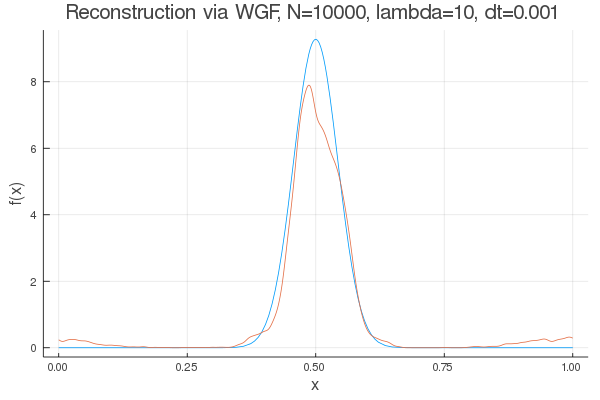
\includegraphics[width = 0.8\textwidth]{analitically_tractable}
%\caption{ }
%\label{fig:at}
%\end{figure}

\subsection{Simulation Study}

\begin{figure}
\centering
\resizebox{0.9\textwidth}{!}{%
\begin{tikzpicture}[baseline, every node/.append]
\node (img1) {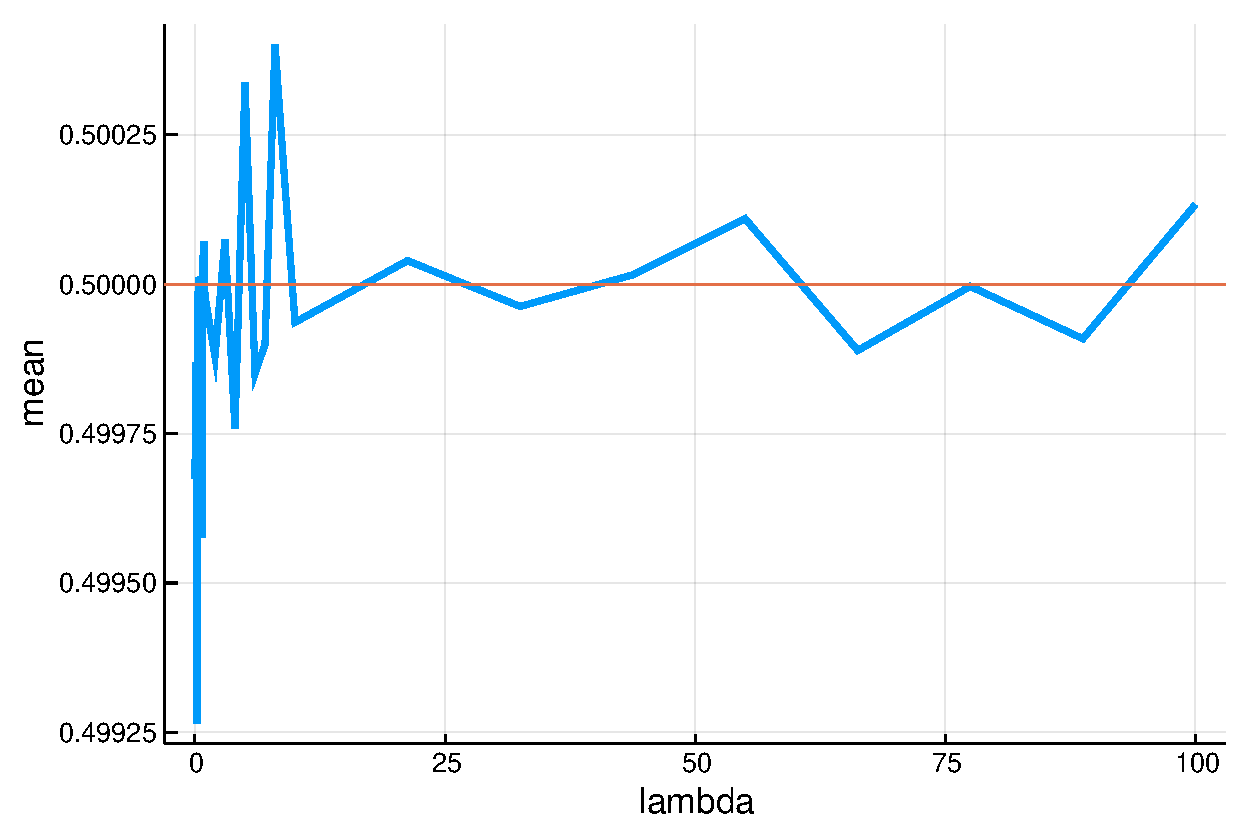
\includegraphics[width=0.40\textwidth]{mean500}};
\node[below=of img1, node distance = 0, yshift = 1cm] (label1){$\lambda$};
  \node[left=of img1, node distance = 0, rotate=90, anchor = center, yshift = -0.7cm] {$\hat{\mu}$};
\end{tikzpicture}
\begin{tikzpicture}[baseline, every node/.append]
\node[right=of img1] (img2) {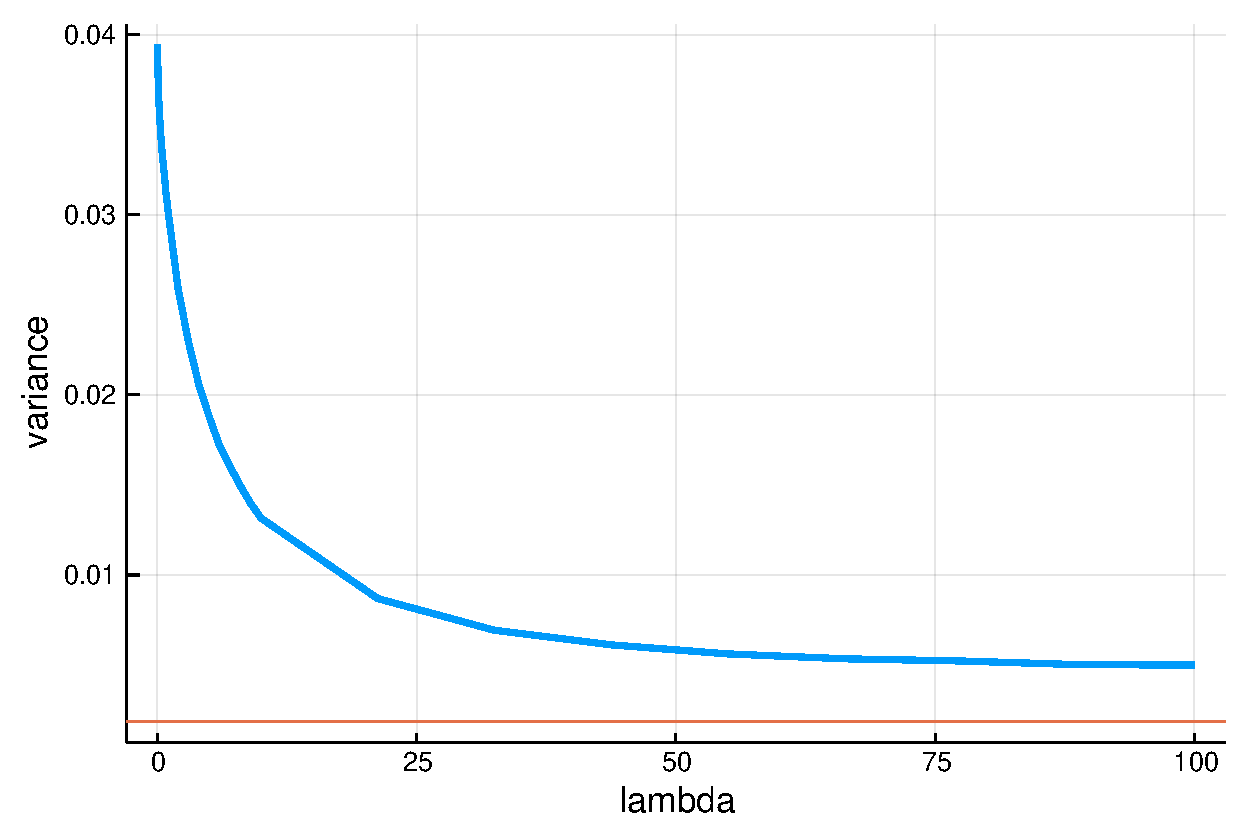
\includegraphics[width=0.40\textwidth]{var500}};
\node[below=of img2, node distance = 0, yshift = 1cm] {$\lambda$};
  \node[left=of img2, node distance = 0, rotate=90, anchor = center, yshift = -0.7cm] {$\hat{\sigma}_\rho^2$};
\end{tikzpicture}
}
\resizebox{0.9\textwidth}{!}{%
\begin{tikzpicture}[baseline, every node/.append]
\node[right=of img2] (img3) {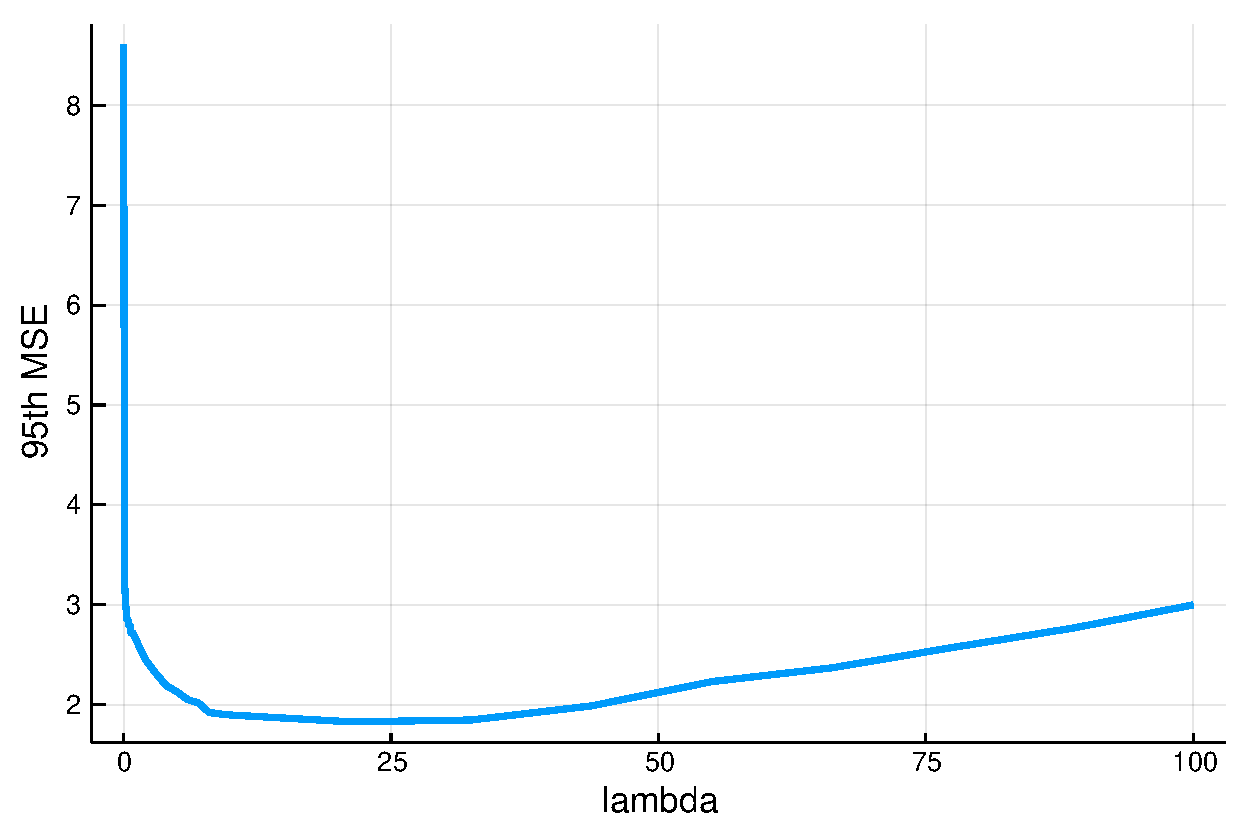
\includegraphics[width=0.40\textwidth]{mse500}};
\node[below=of img3, node distance = 0, yshift = 1cm] {$\lambda$};
  \node[left=of img3, node distance = 0, rotate=90, anchor = center, yshift = -0.7cm] {95th - $\mse$};
\end{tikzpicture}
\begin{tikzpicture}[baseline, every node/.append style={font=\normalsize}]
\node (img5) {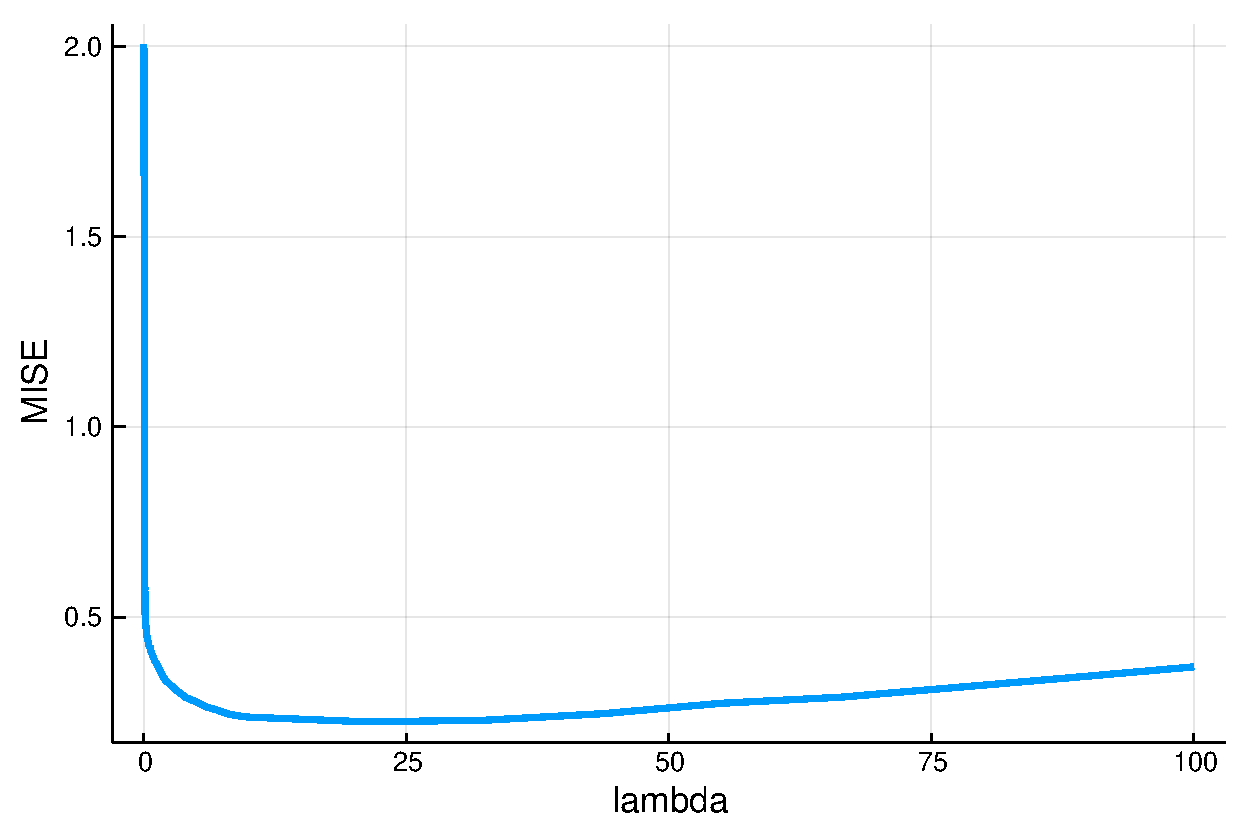
\includegraphics[width=0.40\textwidth]{mise500}};
\node[below=of img5, node distance = 0, yshift = 1cm] {$\lambda$};
  \node[left=of img5, node distance = 0, rotate=90, anchor = center, yshift = -0.7cm] {$\mise$};
\end{tikzpicture}
}
\resizebox{0.9\textwidth}{!}{%
\begin{tikzpicture}[baseline, every node/.append style={font=\normalsize}]
\node[right=of img5] (img6) {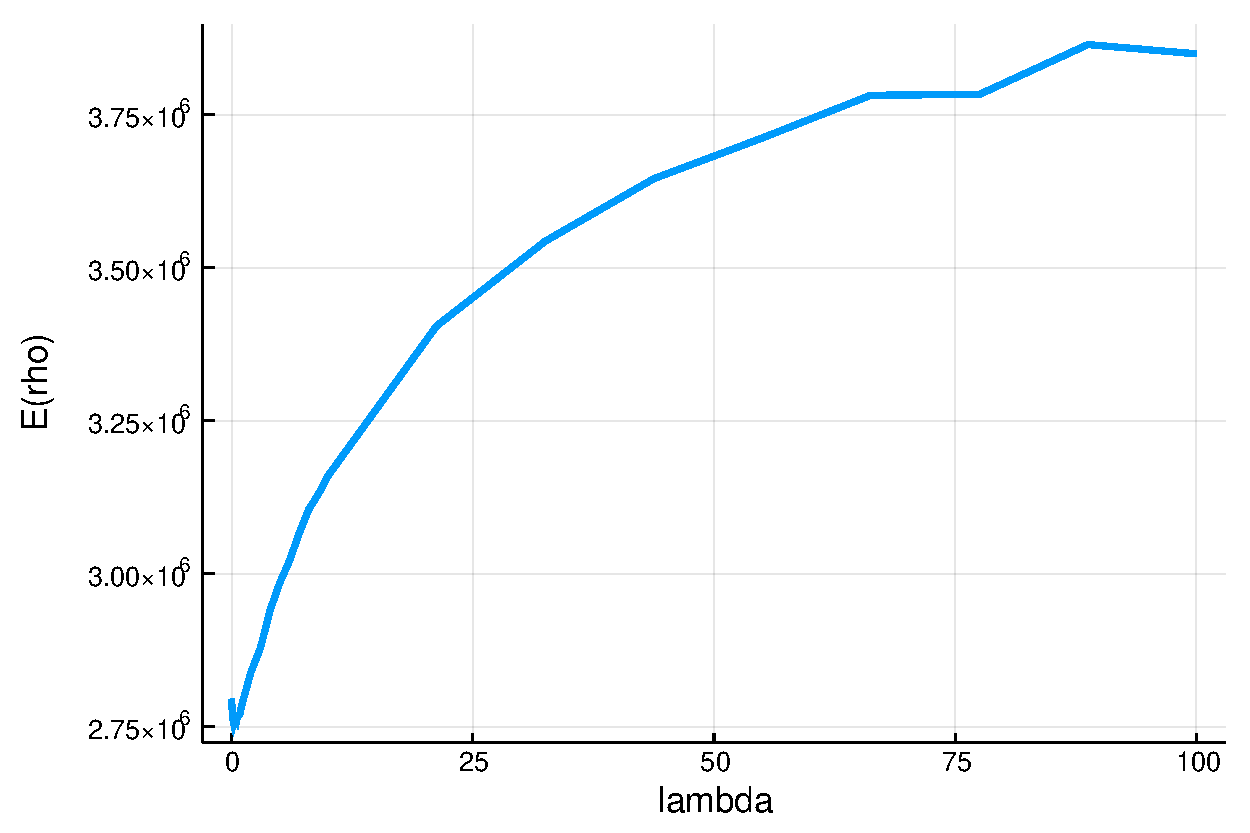
\includegraphics[width=0.40\textwidth]{e500}};
\node[below=of img6, node distance = 0, yshift = 1cm] {$\lambda$};
  \node[left=of img6, node distance = 0, rotate=90, anchor = center, yshift = -0.7cm] {$E(\rho)$};
\end{tikzpicture}
\begin{tikzpicture}[baseline, every node/.append style={font=\normalsize}]
\node[right=of img6] (img7) {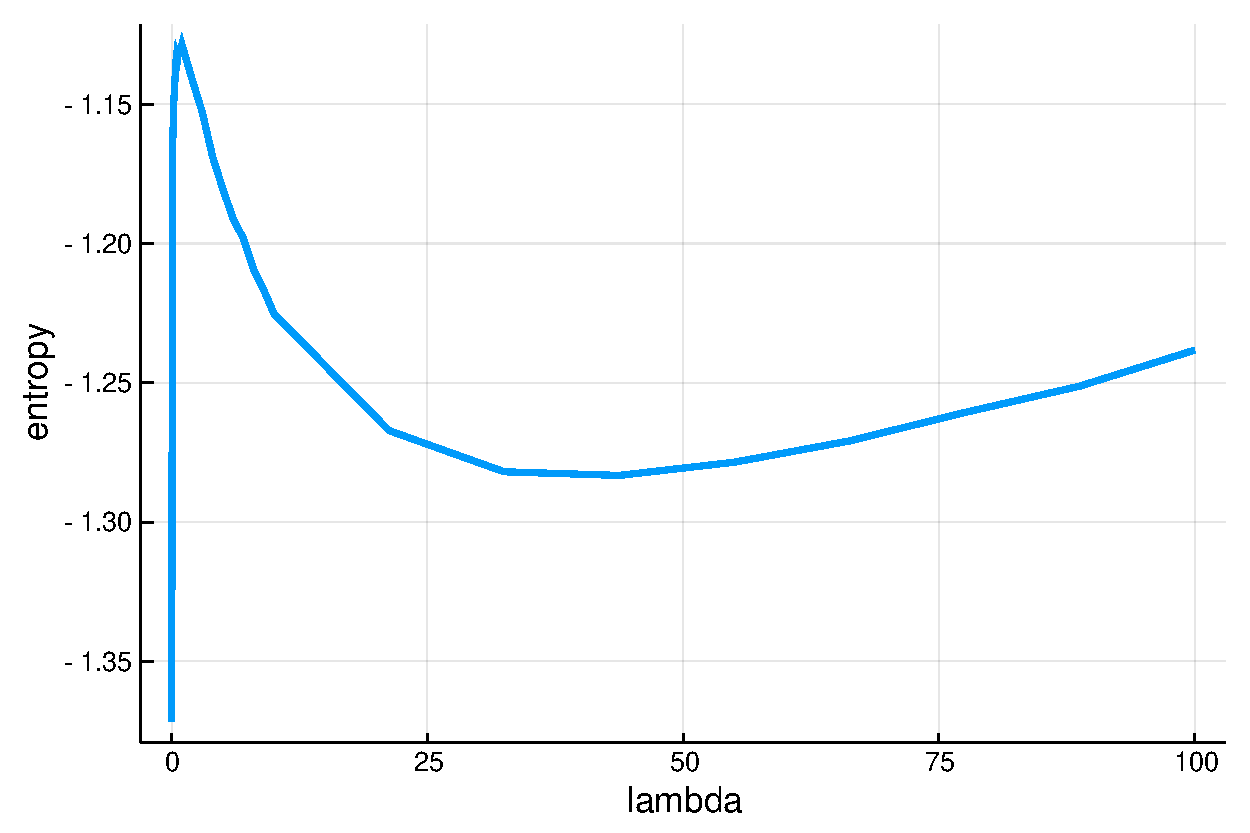
\includegraphics[width=0.40\textwidth]{entropy500}};
\node[below=of img7, node distance = 0, yshift = 1cm] {$\lambda$};
  \node[left=of img7, node distance = 0, rotate=90, anchor = center, yshift = -0.7cm] {$\ent(\rho)$};
\end{tikzpicture}
}
\caption{$N=500$, $dt=10^{-3}$, $T=1$, $\lambda\in[0, 100]$, 1000 repetitions for each $\lambda$}
\end{figure}

%\begin{figure}
%\centering
%\resizebox{0.9\textwidth}{!}{%
%\begin{tikzpicture}[baseline, every node/.append]
%\node (img1) {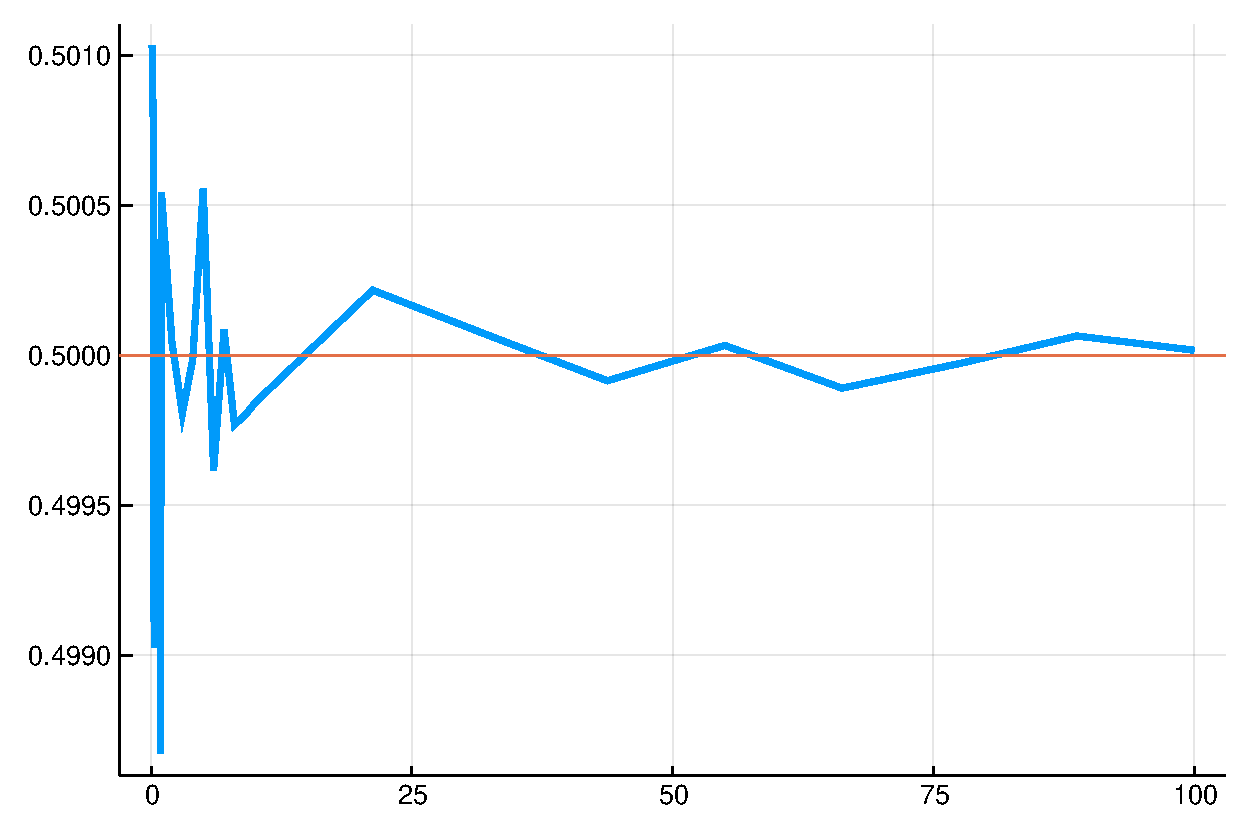
\includegraphics[width=0.40\textwidth]{mean1000}};
%\node[below=of img1, node distance = 0, yshift = 1cm] (label1){$\lambda$};
%  \node[left=of img1, node distance = 0, rotate=90, anchor = center, yshift = -0.7cm] {$\hat{\mu}$};
%\end{tikzpicture}
%\begin{tikzpicture}[baseline, every node/.append style={font=\normalsize}]
%\node[right=of img1] (img2) {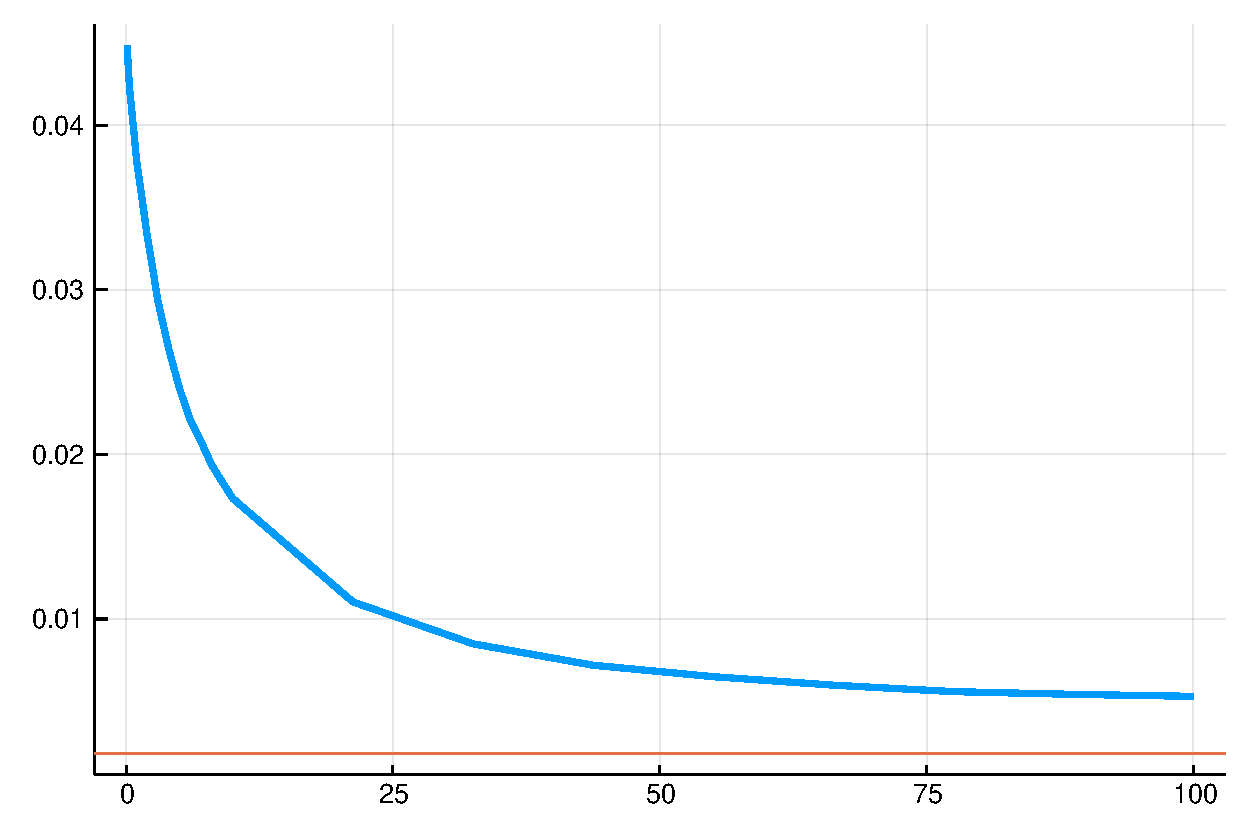
\includegraphics[width=0.40\textwidth]{var1000}};
%\node[below=of img2, node distance = 0, yshift = 1cm] {$\lambda$};
%  \node[left=of img2, node distance = 0, rotate=90, anchor = center, yshift = -0.7cm] {$\hat{\sigma}_\rho^2$};
%\end{tikzpicture}
%}
%\resizebox{0.9\textwidth}{!}{%
%\begin{tikzpicture}[baseline, every node/.append style={font=\normalsize}]
%\node[right=of img2] (img3) {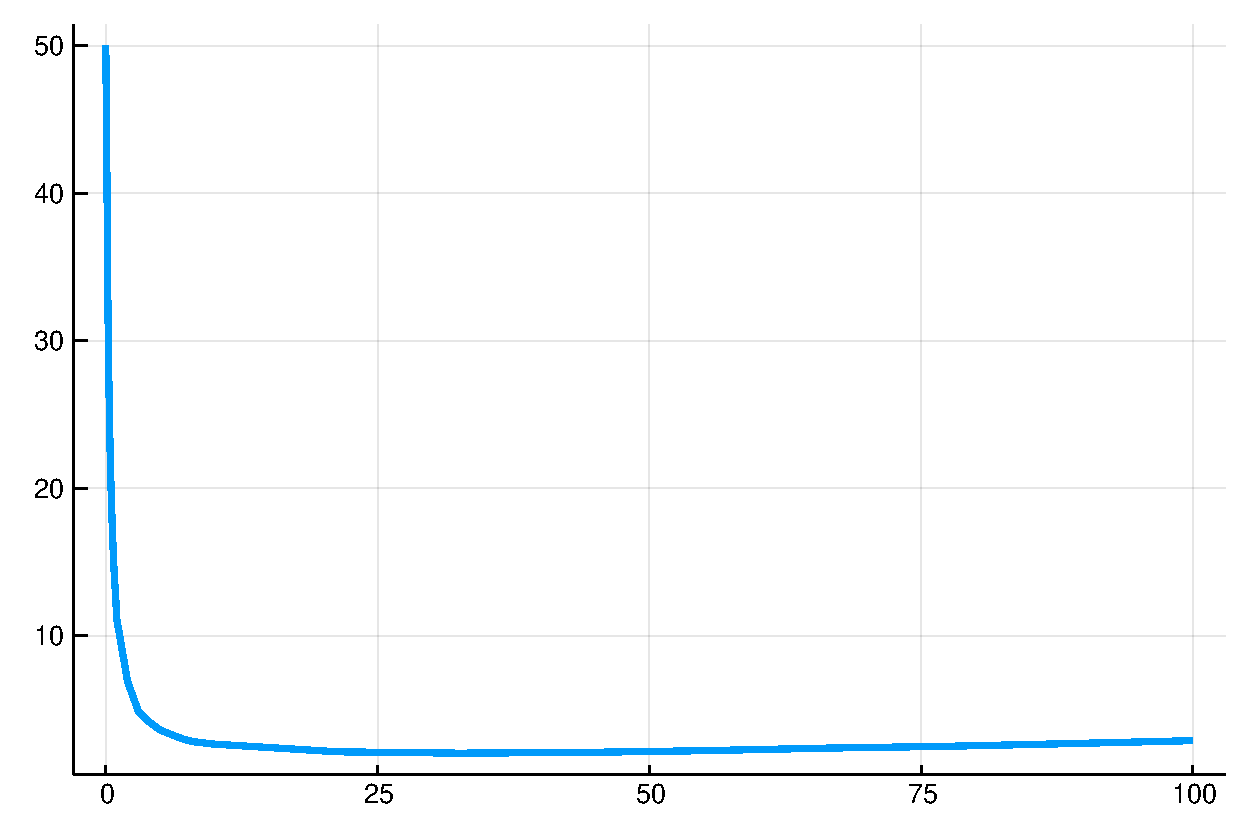
\includegraphics[width=0.40\textwidth]{mse1000}};
%\node[below=of img3, node distance = 0, yshift = 1cm] {$\lambda$};
%  \node[left=of img3, node distance = 0, rotate=90, anchor = center, yshift = -0.7cm] {95th - $\mse$};
%\end{tikzpicture}
%\begin{tikzpicture}[baseline, every node/.append style={font=\normalsize}]
%\node (img5) {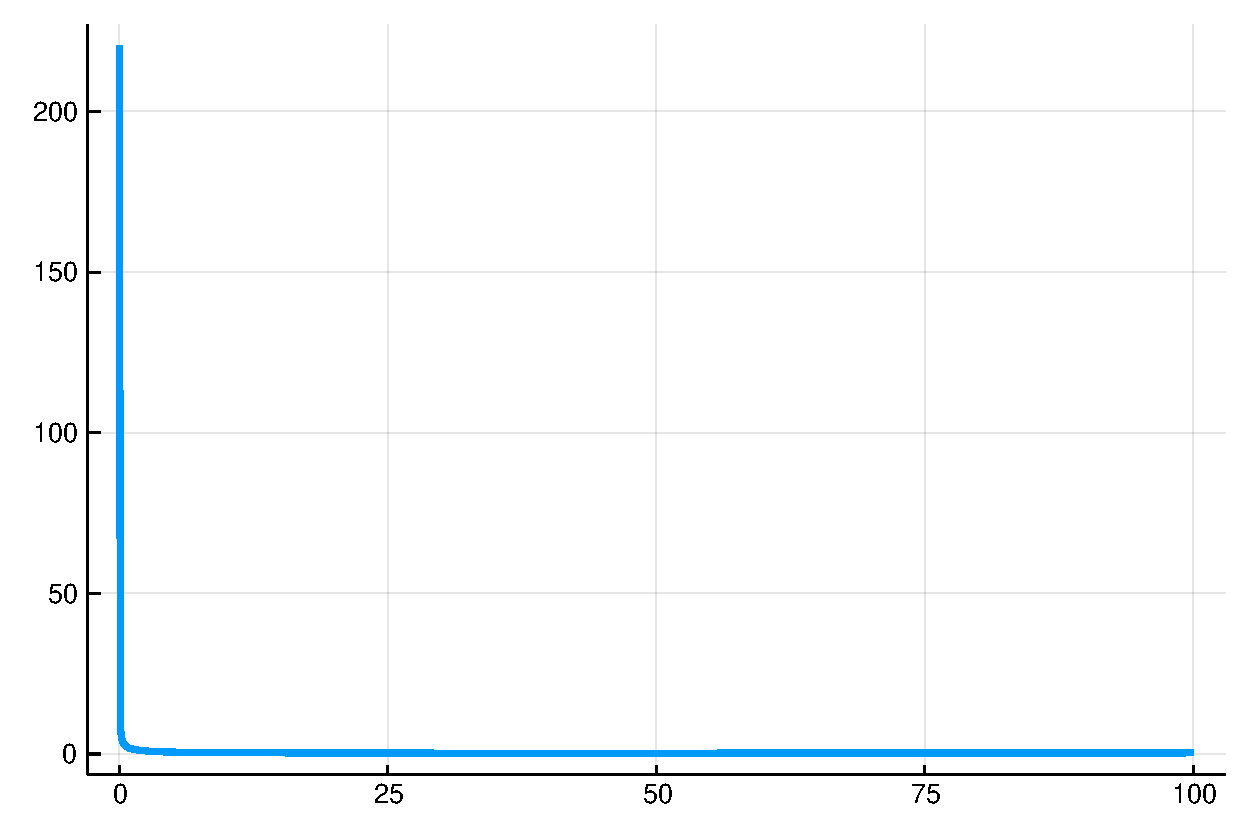
\includegraphics[width=0.40\textwidth]{mise1000}};
%\node[below=of img5, node distance = 0, yshift = 1cm] {$\lambda$};
%  \node[left=of img5, node distance = 0, rotate=90, anchor = center, yshift = -0.7cm] {$\mise$};
%\end{tikzpicture}
%}
%\resizebox{0.9\textwidth}{!}{%
%\begin{tikzpicture}[baseline, every node/.append style={font=\normalsize}]
%\node[right=of img5] (img6) {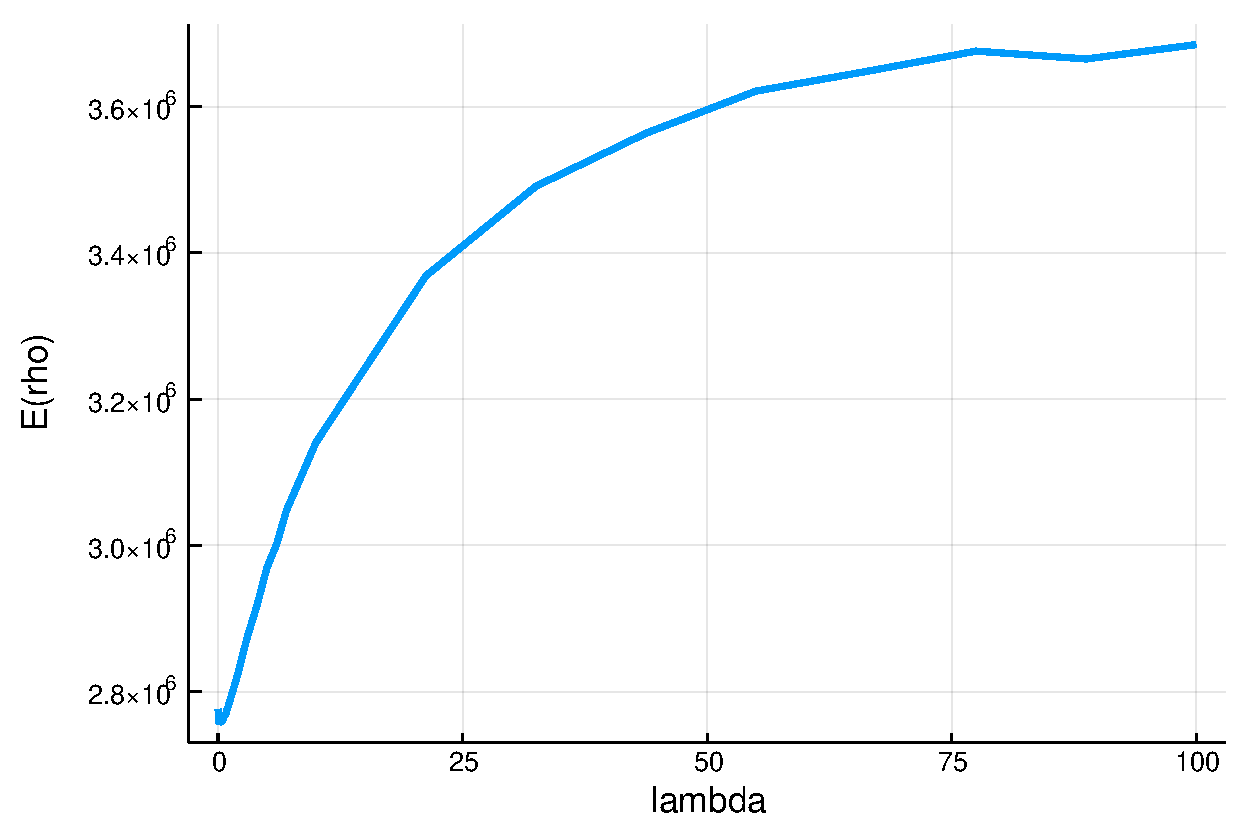
\includegraphics[width=0.40\textwidth]{e1000}};
%\node[below=of img6, node distance = 0, yshift = 1cm] {$\lambda$};
%  \node[left=of img6, node distance = 0, rotate=90, anchor = center, yshift = -0.7cm] {$E(\rho)$};
%\end{tikzpicture}
%\begin{tikzpicture}[baseline, every node/.append style={font=\normalsize}]
%\node[right=of img6] (img7) {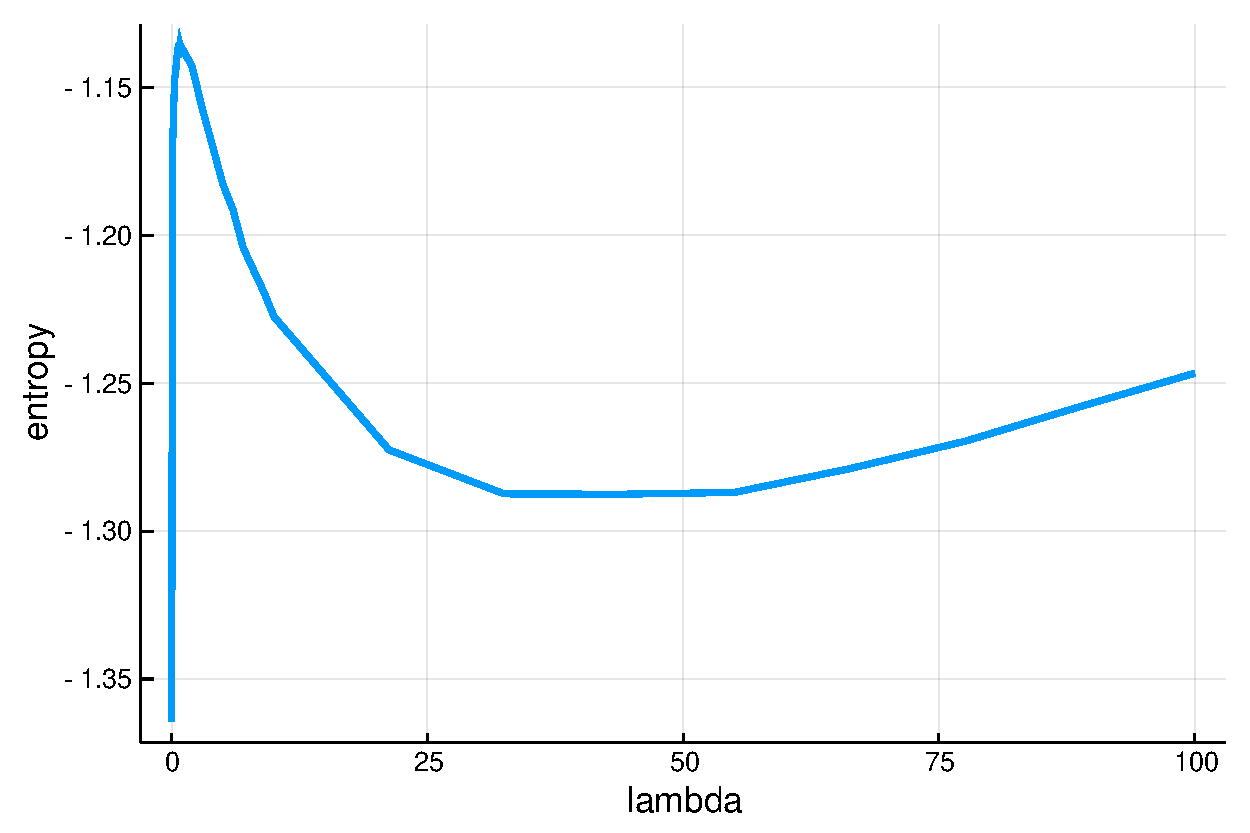
\includegraphics[width=0.40\textwidth]{entropy1000}};
%\node[below=of img7, node distance = 0, yshift = 1cm] {$\lambda$};
%  \node[left=of img7, node distance = 0, rotate=90, anchor = center, yshift = -0.7cm] {$\ent(\rho)$};
%\end{tikzpicture}
%}
%\caption{$N=1000$, $dt=10^{-3}$, $T=1$, $\lambda\in[0, 100]$, 1000 repetitions for each $\lambda$}
%\end{figure}

\section{Gaussian Mixture 1D}
\section{Bivariate Gaussian}
\bibliographystyle{abbrvnat}
\bibliography{wgf_biblio}
\end{document}